% kapitel2.tex
\chapter{Implementierung}
\label{chapter:implementierung}

Nachdem im letzten Kapitel die Konzeption und der Entwurf einer Lösung beschrieben wurde, behandelt dieses Kapitel deren Implementierung. Im Abschnitt \ref{sec:datensatz} wird der Datensatz vorgestellt und aufbereitet. Anschließend werden in den Abschnitten \ref{sec:customNN} und \ref{sec:transferlearning} neuronale Netze mit verschiedenen Ansätzen erstellt, um die Klassifizierung der vier Krankheiten sowie gesunde Blätter zu ermöglichen. Darüber hinaus beschäftigt sich der Abschnitt \ref{sec:voter} mit drei verschiedenen, trainierten Modellen für die Klassifizierung zwischen gesunden Blättern, der Krautfäule und der Dürrfleckenkrankheit.

\section{Datensatz}
\label{sec:datensatz}
Der Datensatz stammt von einer Onlineplattform\cite{plantvillage}, die sich Pflanzengesundheit und -krankheiten widmet. Dabei sammelten die Betreiber der Plattform Daten zu Nutzpflanzen, die frei für jeden zur Verfügung stehen. Diese Daten beinhalten über 150 Pflanzenkulturen sowie 1800 Pflanzenkrankheiten. Von Pflanzenpathologen wurde der Inhalt verfasst und entspricht wissenschaftlichen Anforderungen.

Im Rahmen eines Informatikwettbewerbs von CrowdAI\cite{crowdai} zur Klassifizierung von Pflanzenkrankheiten wurde ein Datensatz erstellt, welcher einer Teilmenge des PlantVillage-Datensatzes entspricht. In der Masterarbeit werden nur die Daten aus dem Wettbewerbs-Datensatz verwendet, welcher in den folgenden Abschnitten vorgestellt wird\cite{dataset}. 

\subsection{Überblick}

Die Bilddaten wurden an experimentellen Forschungsstationen in Kooperation verschiedener staatlicher Universitäten in den USA aufgenommen\cite{dataset}.

Die Pflanzen wurden im Rahmen eines Feldversuchs mit einer Krankheit infiziert. Anschließend wurden die Blätter von Mitarbeitern entfernt und auf ein Papierblatt gelegt. Die Hintergrundfarbe des Papiers war entweder grau oder schwarz. Des Weiteren wurden alle Bilder im Freien aufgenommen. Dabei existieren Unterschiede bei der Lichtintensität. Manche Bilder wurden unter vollem Sonnenlicht und andere Bilder unter bewölkter Lichtbedingungen aufgenommen. Der Zweck hinter diesen verschiedenen Lichtintensitäten liegt darin, dass eine realistische Simulation eines Bauers, der mit dem Smartphone durch das Feld läuft und Bilder aufnimmt, dargestellt werden soll. In der Realität werden Bilder unter einer Reihe von Bedingungen aufgenommen. 

\begin{figure}[h!]
	\centering
	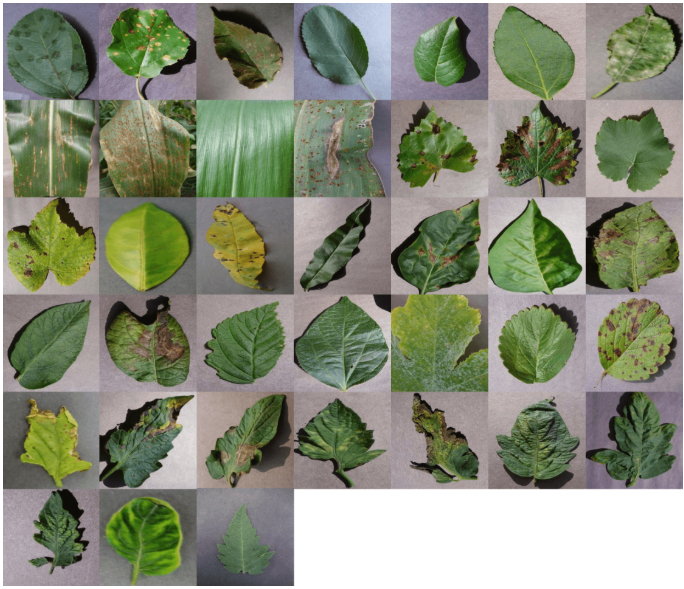
\includegraphics[width=\textwidth]{bilder/data_visualized}
	\caption{Visualisierung der verschiedenen Pflanzenkrankheiten\cite{crowdai}.}
	\label{data_visualized}
\end{figure}
Nach dem erfolgreichen Sammeln wurden die Bilder bearbeitet. Dabei wurde ein Großteil des Hintergrunds entfernt. Des Weiteren wurden die Bilder auf eine Größe von 256 x 256 Pixeln gebracht und sind so ausgerichtet, dass sie nach oben zeigen.

In der Abbildung \ref{data_visualized} werden verschiedene Pflanzen mit unterschiedlichen Krankheiten gezeigt.
In dem Datensatz sind folgende Pflanzen mit der jeweiligen Anzahl von Bilddateien vertreten: Apfel (3172), Heidelbeere (1502), Kirsche (1906), Mais (3852), Traube (4063), Orange (5507), Pfirsich (2657), Paprika (2475), Kartoffel (2152), Himbeere (371), Soja (5090), Kürbis (1835), Erdbeere (1565) und Tomate (18162). Heidelbeere, Himbeere und Soja beinhalten lediglich gesunde Bilddateien. Bei den Pflanzen Orange und Kürbis liegen nur Bilddateien vor, die kranke Blätterausprägungen zeigen. Insgesamt treten in diesem Datensatz 26 Pflanzenkrankheiten auf.

%TODO: Text im Plot größer! Nochmal neu machen!
\begin{figure}[h!]
	\centering
	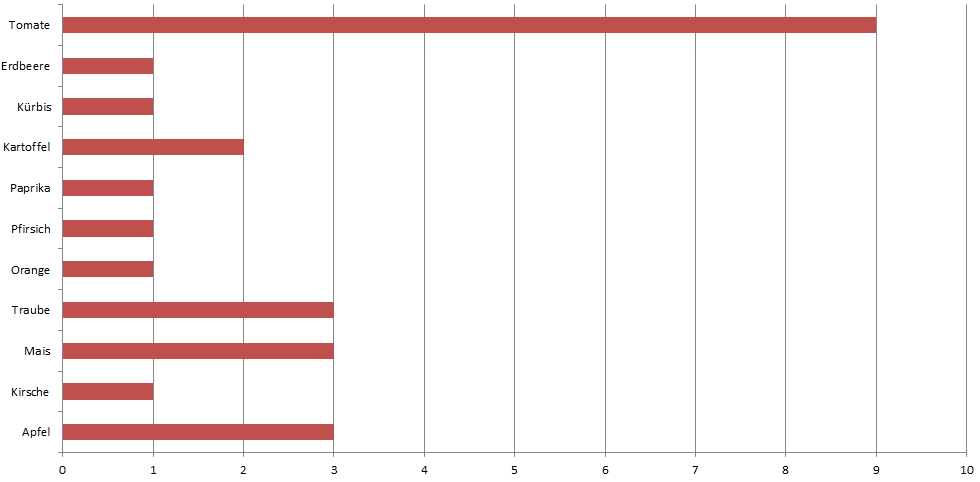
\includegraphics[width=\textwidth]{bilder/disease_distribution}
	\caption{Verteilung der Krankheiten auf Pflanzen (eigene Darstellung).}
	\label{disease_distribution}
\end{figure}

Davon sind 17 Pilzerkrankungen, vier bakteriellen Erkrankungen, zwei Schimmelpilzerkrankungen, zwei Viruserkrankungen und eine Erkrankung durch eine Milbe. In der Abbildung \ref{disease_distribution} wird die Verteilung der jeweiligen Krankheiten auf die Pflanzen veranschaulicht. Dabei sticht die Tomate besonders hervor, da neun Pflanzenkrankheiten in diesem Datensatz zu finden sind.

\begin{figure}[h!]
	\centering
	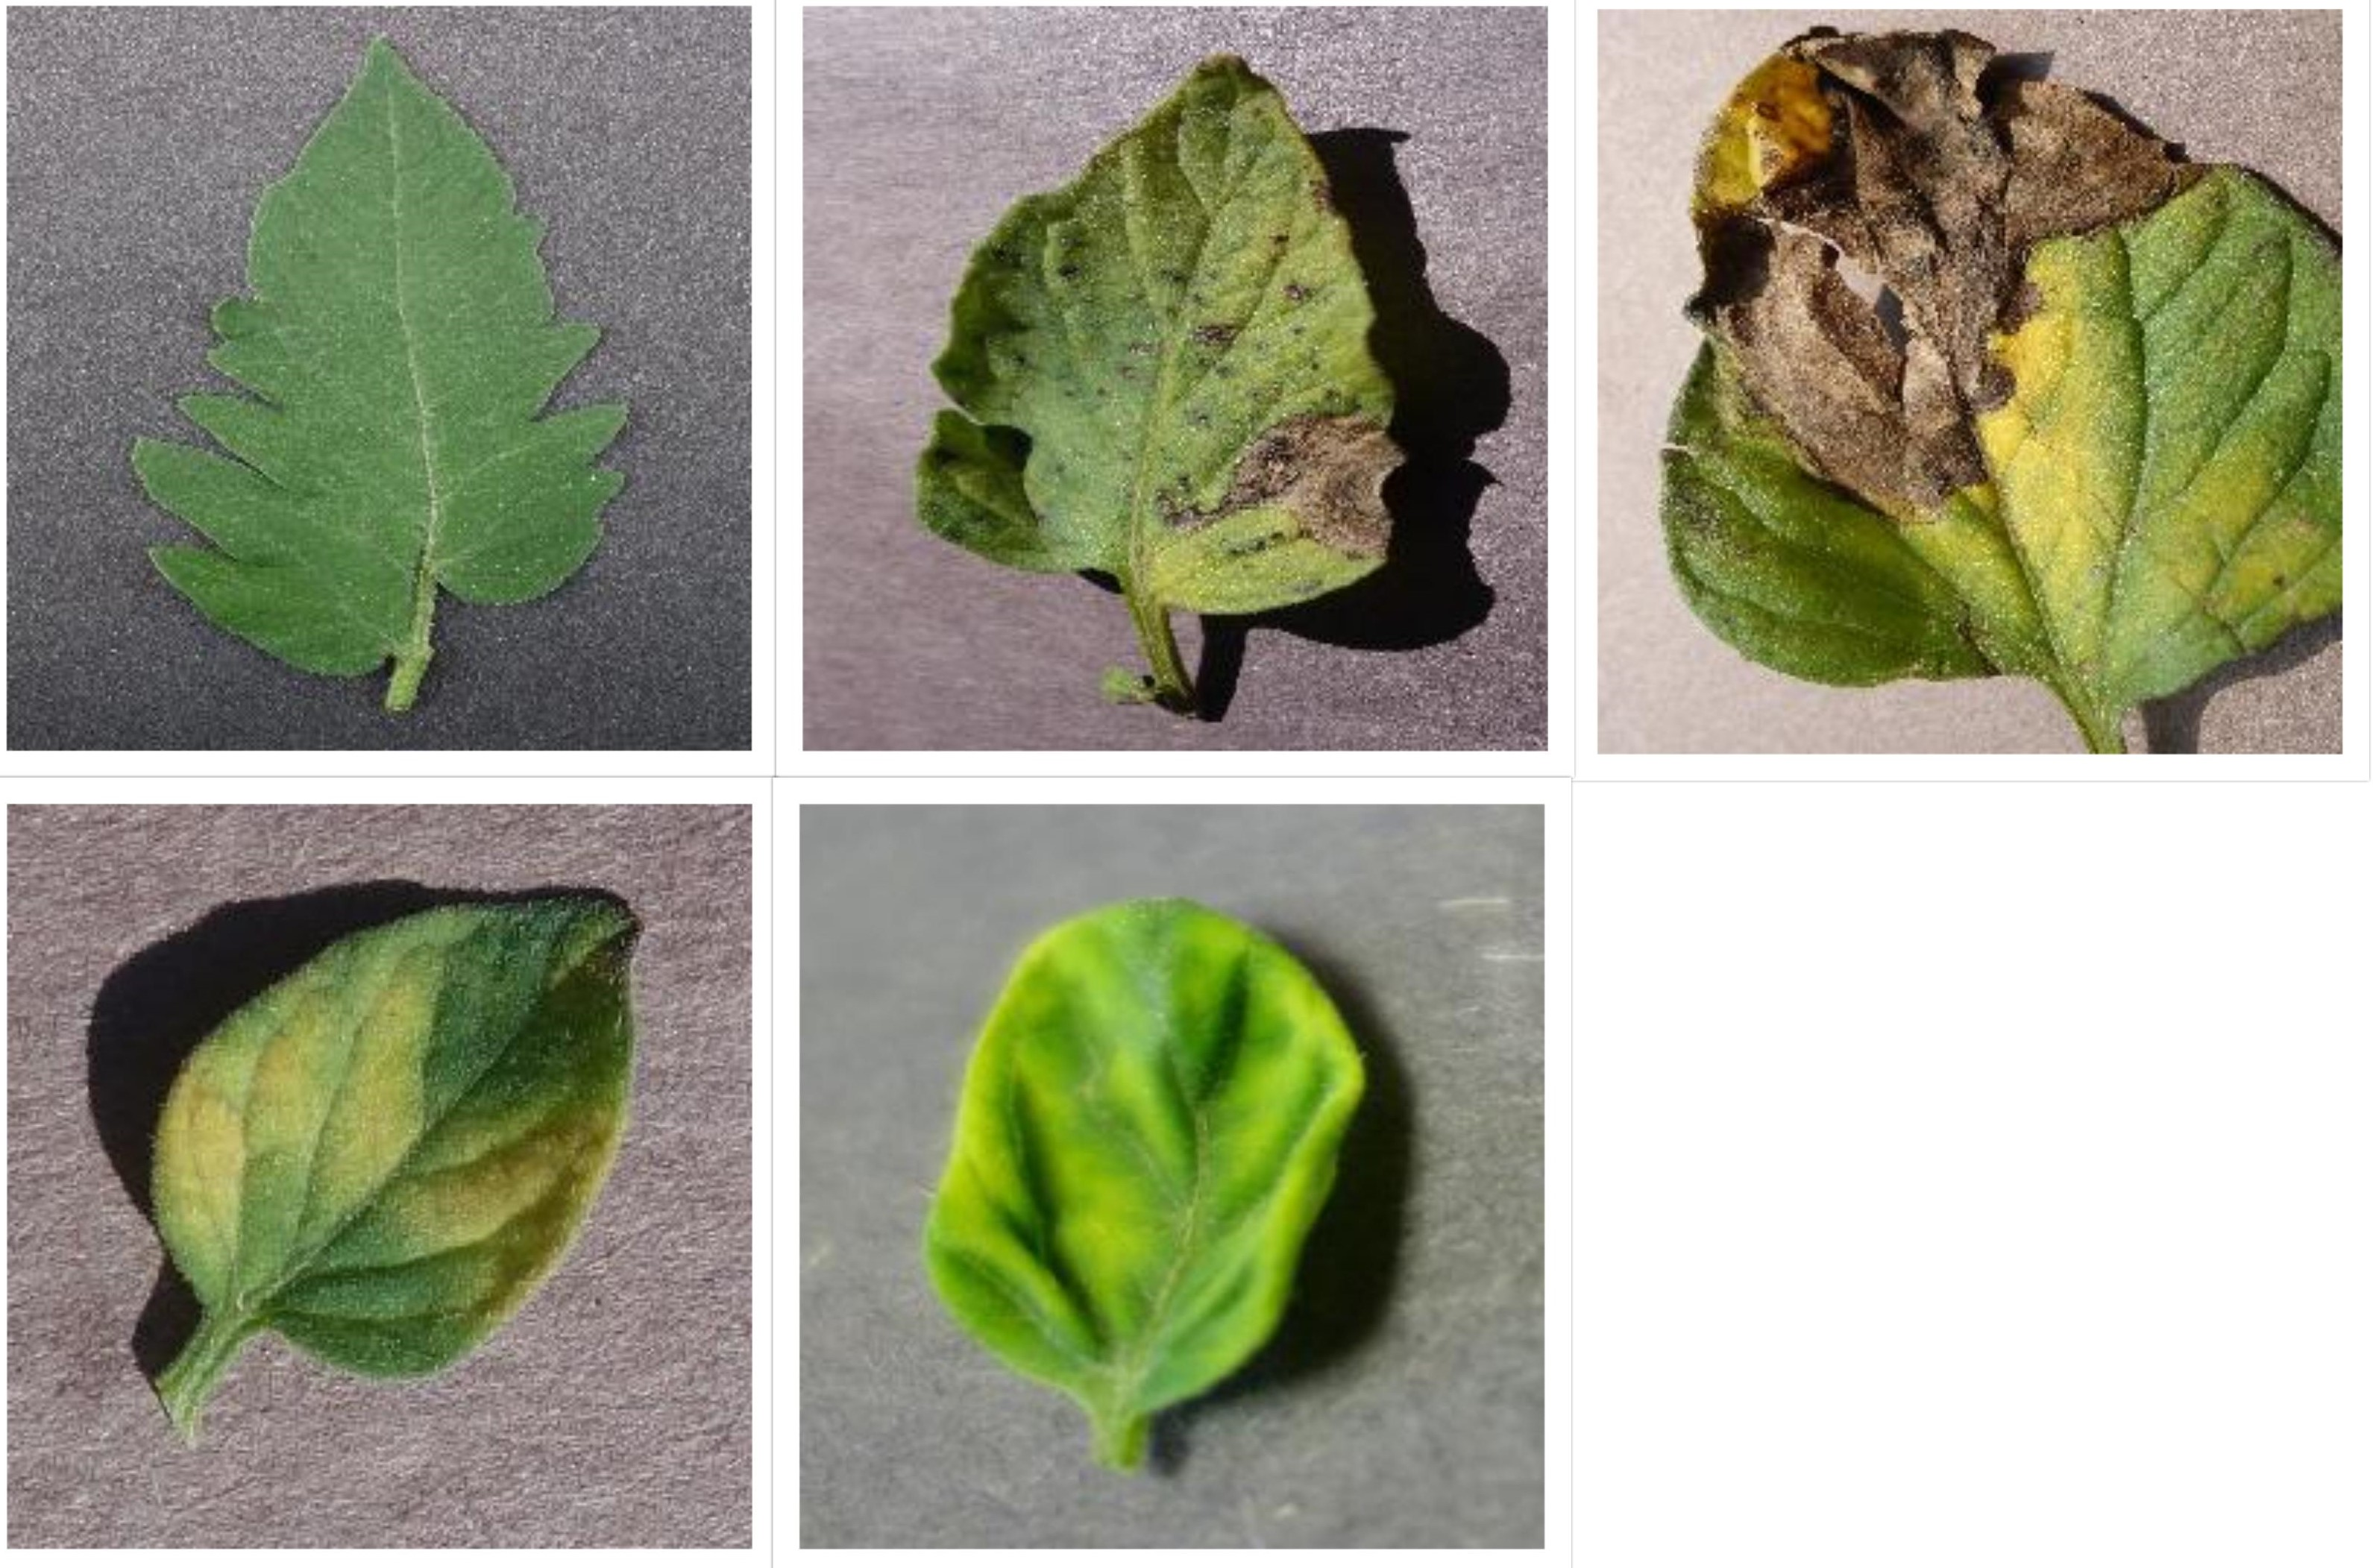
\includegraphics[width=0.8\textwidth]{bilder/collage_5_classes}
	\caption{Visualisierung der fünf Krankheiten, die in dieser Arbeit untersucht wird (eigene Darstellung).}
	\label{collage_5_classes}
\end{figure}


In dieser Masterarbeit wird nur ein Ausschnitt aus dem gegebenen Datensatz behandelt. Fünf Klassen, nämlich \glqq Healthy\grqq, \glqq Early Blight\grqq, \glqq Late Blight\grqq, \glqq Leaf Mold\grqq~und \glqq Yellow Leaf Curl Virus\grqq, werden in der Abbildung \ref{collage_5_classes} beginnend mit der gesunden Tomate von links nach rechts dargestellt. 


\subsection{Aufbereitung}


Neuronale Netze benötigen bestimme Vorverarbeitungsschritte, um gute Ergebnisse liefern zu können. Des Weiteren muss die Struktur des Datensatzes angepasst werden, so dass das Lernverfahren durchführbar ist. 

\subsubsection{Teilung des Datensatzes}
%Quelle wegen den Hauptspeicher
\begin{figure}[!h]
	\begin{minipage}[c]{0.5\textwidth}
		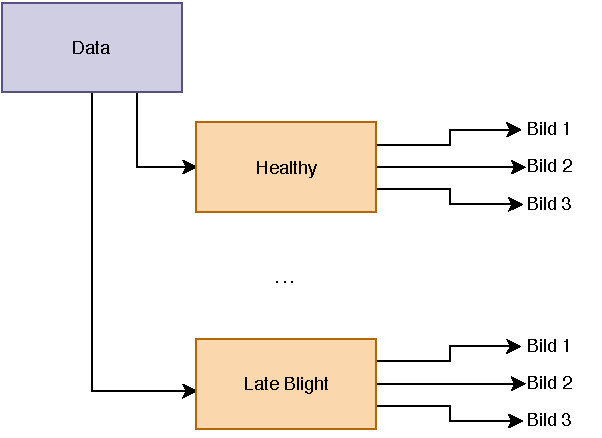
\includegraphics[width=\textwidth]{bilder/original_structure}
		\caption{Die Struktur von dem Datensatz (eigene Darstellung).}
		\label{original_structure}
	\end{minipage}
	\hfill
	\begin{minipage}[c]{0.48\textwidth}
	Der Datensatz hat für jede Klasse einen Ordner. Alle Bilddateien zu einer Klasse befinden sich dementsprechend in einem Ordner. Die Abbildung \ref{original_structure} zeigt die Struktur von dem Datensatz. Für das Trainingsverfahren des neuronalen Netzes wird der Datensatz in Trainings-, Validierungs- und Testsdateien aufgeteilt. Die Abbildung \ref{flow_chart} veranschaulicht die Struktur des Datensatzes, die für die nächsten Schritte benötigt werden.
	\end{minipage}
\end{figure}


Der Vorteil an dieser Strukturierung ist, dass der komplette Datensatz nicht in den 
\begin{figure}[h!]
	\centering
	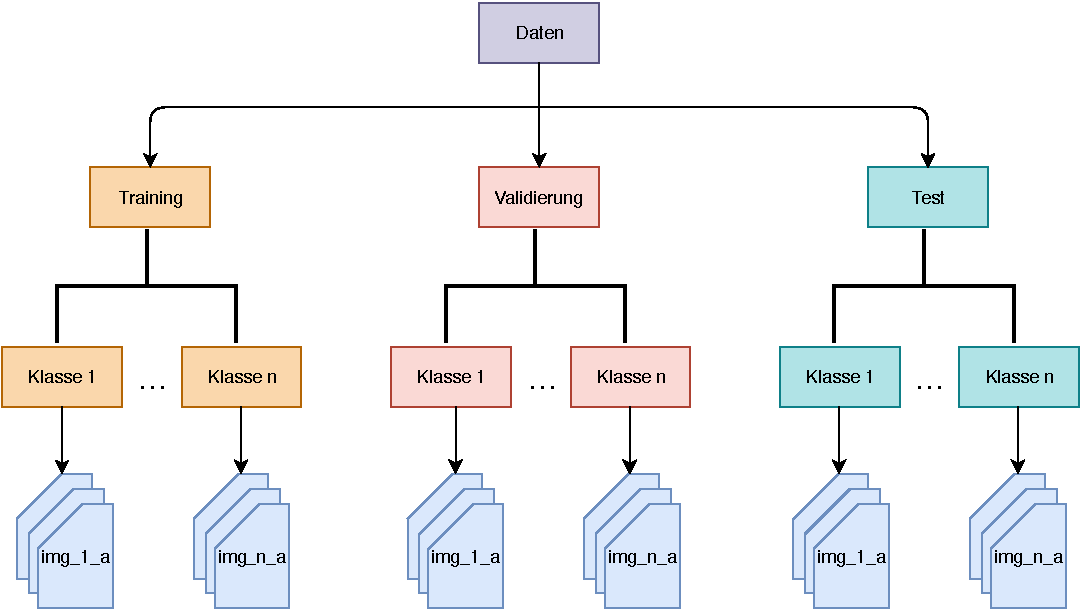
\includegraphics[width=0.73\textwidth]{bilder/flow_chart}
	\caption{Die Darstellung der angepassten Ordnerstruktur, die in drei Teilordner, hier Training, Validierung und Test, aufgeteilt wurde (eigene Darstellung).}
	\label{flow_chart}
\end{figure}

 \newpage~\newline
Hauptspeicher geladen werden muss. Sehr große Datensätze können im schlimmsten Fall nicht im Hauptspeicher passen. Die Bibliothek Keras bietet daher eine Klasse an, die das Einlesen der Daten übernimmt. Die Klasse \textit{ImageDataGenerator}\cite{flowfrom} liest schrittweise die Daten ein. Dabei werden die Daten stapelweise (engl. Batch) eingelesen, so dass kleinere sowie sehr große Datensätze verwendet werden können. Es werden nur so viele Daten in den Hauptspeicher geladen, wie für den aktuellen Batch beim Training und der Validierung des Modells benötigt werden.

\subsubsection{Anpassung der Verteilung}

CNNs haben in der Praxisanwendung Probleme, wenn einige Klassen eine deutlich höhere Anzahl an Daten in dem Trainingsdatensatz als andere Klassen haben. Dieses Klassenungleichgewicht sorgt für Schwierigkeiten bei dem Lernverfahren von klassischen Klassifikatoren und mehrschichtigen neuronalen Netzen. Dabei wirkt es sich die Konvergenz während der Trainingsphase aus und könnte die Generalisierung des Modells bei dem Testdatensatz negativ beeinflussen. Eine naive, leichte Lösung des Problems ist das Undersampling. Mit dieser Methodik wird zufällig ein Teil der Daten aus den überrepräsentierten Klassen entfernt\cite{papernn}.

\begin{figure}[h!]
	\centering
	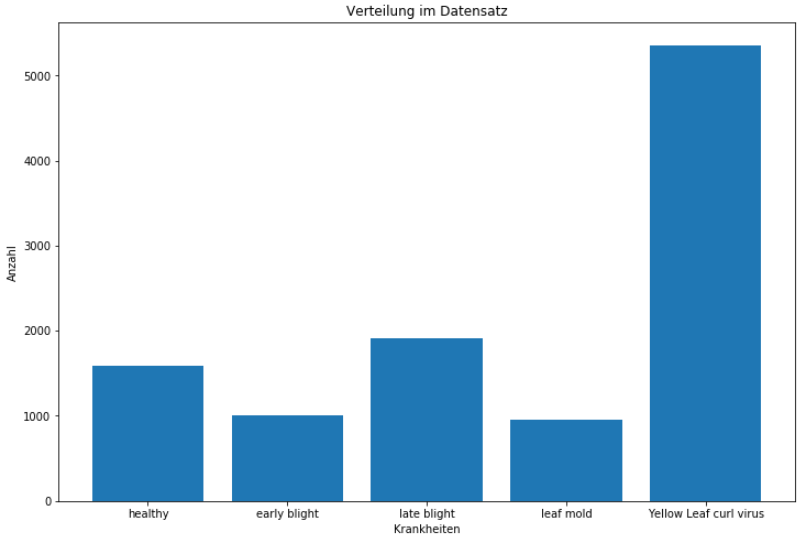
\includegraphics[width=\textwidth]{bilder/original_distribution.PNG}
	\caption{Die Verteilung der Daten ist bei den Klassen nicht gleich verteilt. Die Datenmenge von der TYLCV-Krankheit ist mindestens doppelt so groß im Vergleich zu den anderen Krankheiten (eigene Darstellung).}
	\label{original_distribution}
\end{figure}

In der Abbildung \ref{original_distribution} wird die momentane Verteilung der Daten von vier verschiedenen Pflanzenkrankheiten sowie der gesunden Klasse veranschaulicht. Hierbei ist klar zu sehen, dass die Klasse \glqq TYLCV\grqq~mit über 5000 Bilddaten deutlich überrepräsentiert ist. Die anderen Klassen haben eine Datenmenge zwischen 800 und 2000 Bildern. Daher wird hier der naive Ansatz angewendet, um alle Datenmengen jeweiliger Klasse auf den Bereich 700 bis 800 zu reduzieren. Die Trainingsdaten der Klasse \glqq TYLCV\grqq~werden drastisch gekürzt. Des Weiteren wurden die beiden leicht überrepräsentierten Klassen \glqq healthy\grqq~und \glqq leaf mold\grqq~auch gekürzt. Nun befindet sich die Menge von Trainingsdaten aller Klassen in der Spannweite zwischen 700 und 800 (s. Abbildung \ref{corrected_distribution}). Außerdem wurde in dieser Abbildung die Anzahl der Validierungs- und Testdaten in orange und grün gekennzeichnet. Die Menge an Validierungsdaten liegt zwischen 150 bis 300. Die Testdaten sind im Vergleich zu den anderen Daten deutlich geringer, nämlich zwischen 80 bis 280.

\begin{figure}[h!]
	\centering
	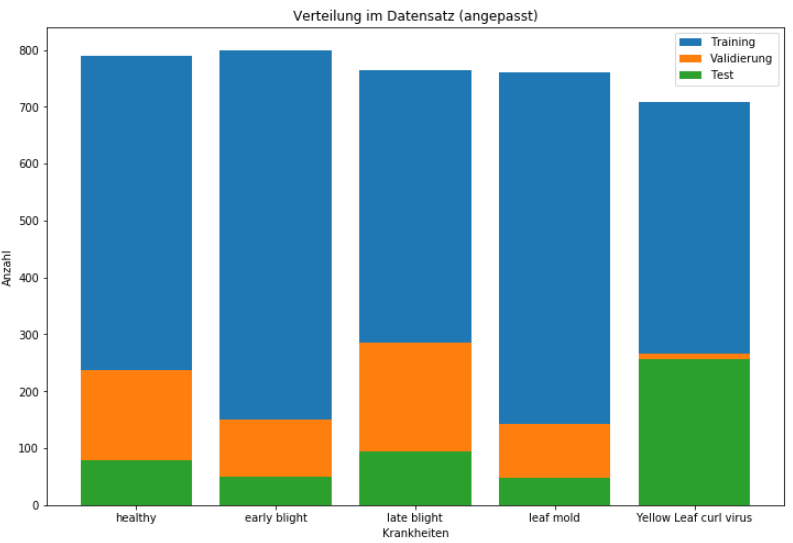
\includegraphics[width=\textwidth]{bilder/corrected_distribution.PNG}
	\caption{Die Anzahl der Trainingsdaten von allen Klassen (blau) befindet sich in dem Bereich zwischen 700 und 800. Die orangene Säule repräsentiert die Validierungsdaten, dessen Anzahl maximal 280 liegt. Außerdem stellt die grüne Säule die Testdaten dar, die bei der Klasse \glqq TYLCV\grqq~leicht höher ist (eigene Darstellung).}
	\label{corrected_distribution}
\end{figure}


\subsubsection{Vorverarbeitung}

%load the data from the directory on demand with the help of flow_from_directory in Keras
% https://keras.io/preprocessing/image/#imagedatagenerator-class

Da der Datensatz nicht vorverarbeitet ist, werden Vorverarbeitungen benötigt, um den Datensatz optimal für den Lernprozess vorzubereiten. Zunächst wird der Datensatz künstlich erweitert, um eine Anzahl von Variationen zu erzeugen. Damit kann eine Überanpassung des Modells verhindert werden. Der Gradbereich für zufällige Rotationen liegt bei maximalen 40 Grad. Darüber hinaus werden die Bilder horizontal und vertikal in beide Richtungen zufällig bis 20\% verschoben. Außerdem werden die Bilder im Gegenuhrzeigersinn um 20\% geschert. Um weitere Diversität in dem Datensatz zu erzeugen, werden die Bilder mit dem Faktor 30\% rein- sowie rausgezoomt. Die durch Transformation entstandenen Flächen werden mit dem Farbton des angrenzenden Pixels gefüllt. Ein weiterer Vorverarbeitungsschritt ist nun das zufällige, horizontale Spiegeln der Bilder. Anschließend werden die Farbwerte normiert. Da jeder Farbkanal jeweils acht Bit lang ist, ist der maximale Wert bei 256. Daher werden die Farbwerte durch 255 geteilt, um den Zahlenbereich der RGB-Werte zwischen null und eins zu erhalten. 

In Abbildung \ref{data_segm} werden drei Bilder gezeigt. Das linke Bild ist das unverarbeitete Bild aus dem Datensatz. Die Bilder, die sich in der Mitte sowie rechts befinden, wurden mit verschiedenen Transformationen geändert. Das mittlere Bild ist horizontal gespiegelt und die Blattfläche nimmt mehr Platz in dem Bild ein. Deutlich ist es zu erkennen, dass das rechte Bild herausgezoomt wurde. Daher hat dieses Bild einige geradlinige Füllelemente.  

%Vorher und nachher Vergleich
\begin{figure}[h!]
	\centering
	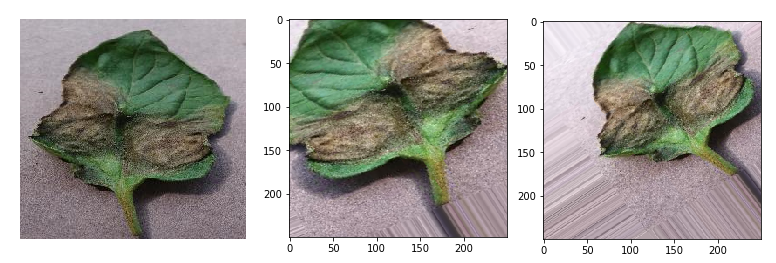
\includegraphics[width=\textwidth]{bilder/data_segmentation.PNG}
	\caption{Das linke Bild zeigt das unveränderte Bild. Durch Transformationen wird das mittlere sowie rechte Bild verändert. Des Weiteren wurden die Farbweite von den beiden Bildern normalisiert.}
	\label{data_segm}
\end{figure}

\section{Anmerkungen zum Training}
%Titel ändern??

Aus Übersichtlichkeitsgründen wird ein Teil der Hyperparameter für alle folgenden Modelle hier zusammengefasst, da sie größtenteils redundant sind. Bei allen Modellen greift das Modell auf die kategorische Kreuzentropie als Kostenfunktion zurück, da das Klassifizierungsproblem mehr als zwei Klassen beinhaltet. Des Weiteren werden die neuronalen Netze mithilfe von dem Gradientenabstieg des Typs \glqq Adam\grqq~trainiert. Hierbei ist die Lernrate auf den Wert 0.001 gesetzt. Die Größe des Batchs liegt bei 230. 

Unterschiede zwischen den Modellen liegen bei der Anzahl der Epochen oder der Konfiguration des frühzeitigen Abbruchs des Trainings.

\section{Aufbau des neuronalen Netzes}
\label{sec:customNN}
%Chapter Titel anpassen?
%Convolution und poolingschicht schreibweise nochmal überprüfen

Das hier vorgestellte neuronale Netz soll die vier Krankheiten und zusätzlich gesunde Blätter erkennen, die im Abschnitt \ref{sec:Blattkrankheiten} vorgestellt wurden.  

%Modell
%\subsection{Struktur}
Das Modell hat eine grundlegende Struktur. Nach jeder Faltungsschicht folgt unmittelbar eine Max-Poolingschicht. Insgesamt treten solche Konstrukte fünf mal auf. Anschließend beinhaltet das Modell zwei weitere voll verbundene Schichten. Grundsätzlich haben alle Filter in den Faltungsschichten die Größe 3 x 3 und werden mit der ReLU-Aktivierungsfunktion aktiviert. Die Fenstergröße der Poolingschichten ist auf die Größe 2 x 2 gesetzt.
In Abbildung \ref{my_arch} wird die Struktur des Modells visualisiert. Gelbe Flächen sollen Faltungsschichten, rote Poolingsschichten und blaue dementsprechend Dropout-Schichten symbolisieren. Zunächst wird das Modell mit einer Faltungsschicht, die das Eingangsbild in der Größe 150 x 150 akzeptiert, beginnen. Das Eingangsbild wurde von der ursprünglichen Größe von 256 x 256 auf 150 x 150 verkleinert, um in der Lernphase Zeit zu sparen. Die Anzahl der Filter in der ersten Faltungsschicht beträgt 32.

\begin{figure}[h!]
	\centering
	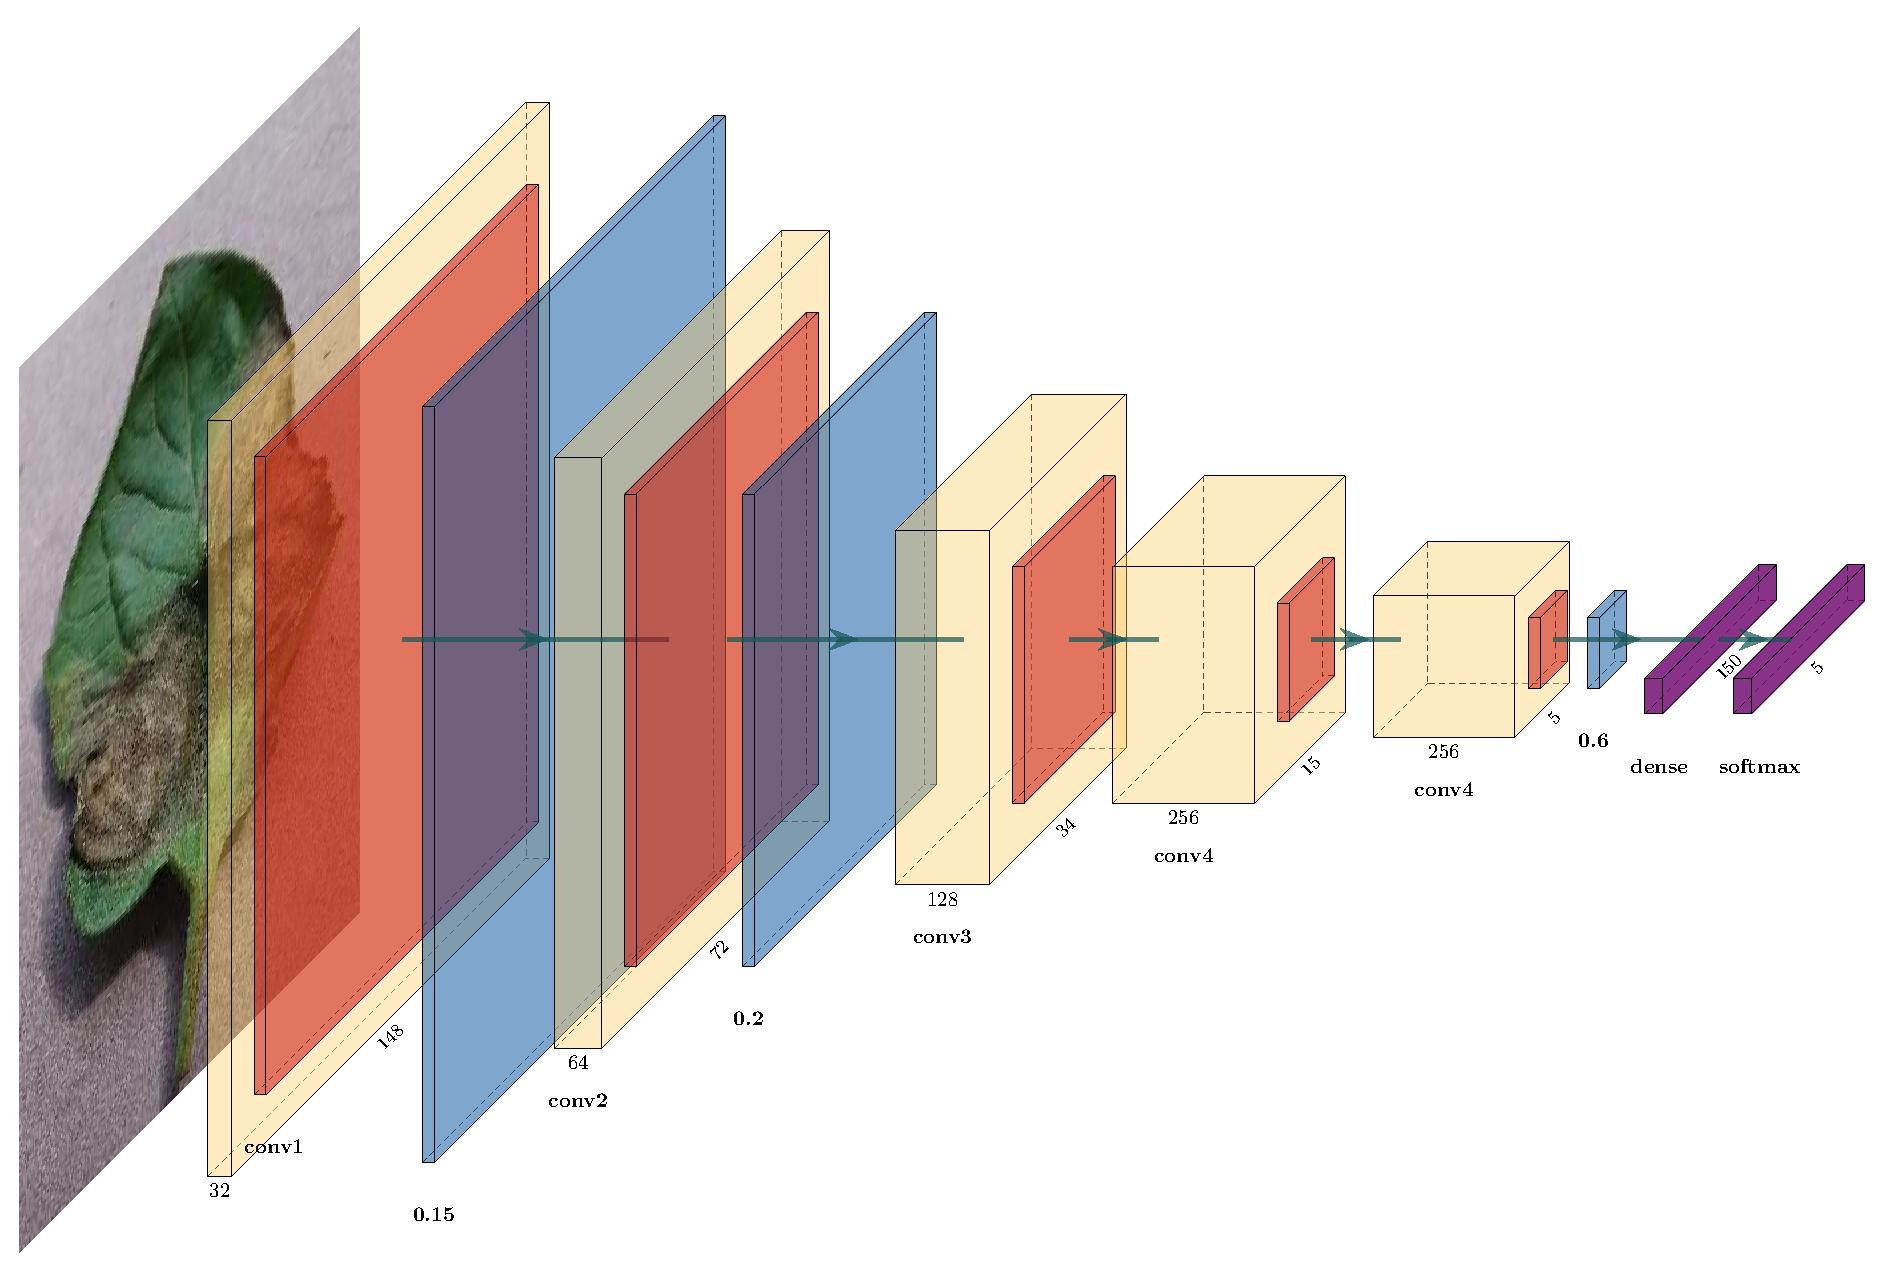
\includegraphics[width=\textwidth]{bilder/my_arch.pdf}
	\caption{Darstellung des Modells mit fünf Faltungs- und Poolingschichten (eigene Darstellung).}
	\label{my_arch}
\end{figure} 
 
Nach der ersten Max-Poolingschicht folgt die erste Dropout-Schicht mit dem Wert 0.15. Anschließend folgt die zweite Faltungsschicht mit 64 Filtern. Auch hier wird nach der zweiten Max-Poolingschicht eine zweite Dropout-Schicht hinzugefügt, um 20\% der Ausgabefunktionen auf den Wert 0 setzen zu können. Die dritte Faltungsschicht hat insgesamt 128 Filter. Anknüpfend werden zwei weitere Faltungsschichten mit ihren Max-Poolingschichten im Modell hinzugefügt. Hierbei beträgt die Anzahl der Filter bei beiden Schichten 256. Daraufhin fügt sich eine Dropout-Schicht an, die auf 60\% eingestellt ist. Nach der letzten Dropout-Schicht weist das Modell zwei voll verbundene Schichten auf, wobei die erste Schicht 150 Knoten und die ReLU-Aktivierungsfunktion hat. Außerdem werden die Gewichte dieser Schicht mit einer L2-Regularisierung mit dem Faktor 0.002 angepasst. Die zweite voll verbundene Schicht hat nur fünf Knoten, da nur fünf Klassen klassifiziert werden sollen. Um die Klassifikation durchführen zu können, wird auf die Softmax-Aktivierungsfunktion zurückgegriffen. 




\paragraph{Training}
~\newline

Das Modell wird mit 200 Epochen trainiert. Dabei kann das Training frühzeitig abgebrochen werden, wenn sich die Kosten des Validierungsdatensatzes nicht minimieren. Bevor der Abbruch stattfindet, werden zunächst 20 Epochen durchlaufen. Hierbei stellt sich heraus, ob die Kostenfunktion einen neuen minimalen Wert zurückgibt. Das Trainingsverfahren bricht bei der Hälfte, hier bei der 96. Epoche, schon ab. Das beste Modell bezüglich der minimalen Kosten wurde in der 76. Epoche erreicht und hat eine Genauigkeit von 98.51\%.







\section{Voter}
\label{sec:voter}
%- performance des Voters im  kapitel eval
Um die Anzahl der Fehlklassifizierungen reduzieren zu können, wird in diesem Abschnitt auf einen Voter gesetzt. Die Grundidee hierbei ist, dass mehrere Modelle dasselbe Eingangsbild erhalten und klassifizieren. Der Voter wählt aus den Ergebnissen der drei verschiedenen trainierten Modelle die passende Klasse aus. Hierbei wird die Klasse, die am häufigsten unter den drei Modellen erkannt wurde, ausgewählt. Die folgenden Modelle wurden speziell für die zwei Krankheiten, hier Dürrfleckenkrankheit und Krautfäule, entworfen. Daher kann der Voter zwischen diesen beiden Krankheiten sowie gesunden Blättern auswählen.


\subsection{Modell 1}
\label{model1_voter}
%\subsubsection{Struktur}
Das vorliegende Modell sowie alle anderen folgenden Modelle beinhalten denselben Aufbau. Auf jede Faltungsschicht folgt eine Max-Poolingschicht. Diese Kombination tritt genau vier Mal auf. Zwei voll verbundene Schichten runden die Architektur des Modells ab. Auch hier ist die Filtergröße der Faltungsschichten 3 x 3 groß und sind mit der ReLU-Aktivierungsfunktion eingestellt. Die Größe des Max-Poolingfenster beträgt  2 x 2. Diese Parametergrößen sind bei den folgenden Modellen in den Abschnitten \ref{model2_voter} und \ref{model3_voter} dieselben. 
Die erste Faltungsschicht mit 64 Filtern akzeptiert das Eingangsbild, das in der Größe 150 x 150 vorliegt. Anschließend wurde nach der Max-Poolingschicht eine Dropout-Schicht hinzugefügt, welche 15\% der Ausgabefunktionen nicht mehr beachtet. Nach einer solchen Dropout-Schicht wird eine Kombination aus einer Faltungsschicht mit der doppelten Anzahl von Filtern und einer Max-Poolingschicht gesetzt. Daraufhin folgt wieder eine Dropout-Schicht, die auf 20\% eingestellt ist. Nach dieser Schicht wird die Architektur mit zwei Kombinationen aus einer Faltungschicht mit 256 Filtern und einer Max-Poolingschicht erweitert. Nach der Erweiterung wird eine letzte Dropout-Schicht mit der Rate von 60\% ergänzt, so dass zwei voll verbundene Schichten mit 150 sowie fünf Knoten vervollständigt werden können. Die erste voll verbundene Schicht weist die ReLU-Aktivierungsfunktion auf. Die Gewichte in dieser Schicht werden mit dem Faktor 0.002 mittels einer L2-Regularisierung korrigiert. Die zweite voll verbundene Schicht ist mit einer Softmax-Aktivierungsfunktion versehen, um die drei Klassen bestimmen zu können.        


\begin{figure}[h!]
	\centering
	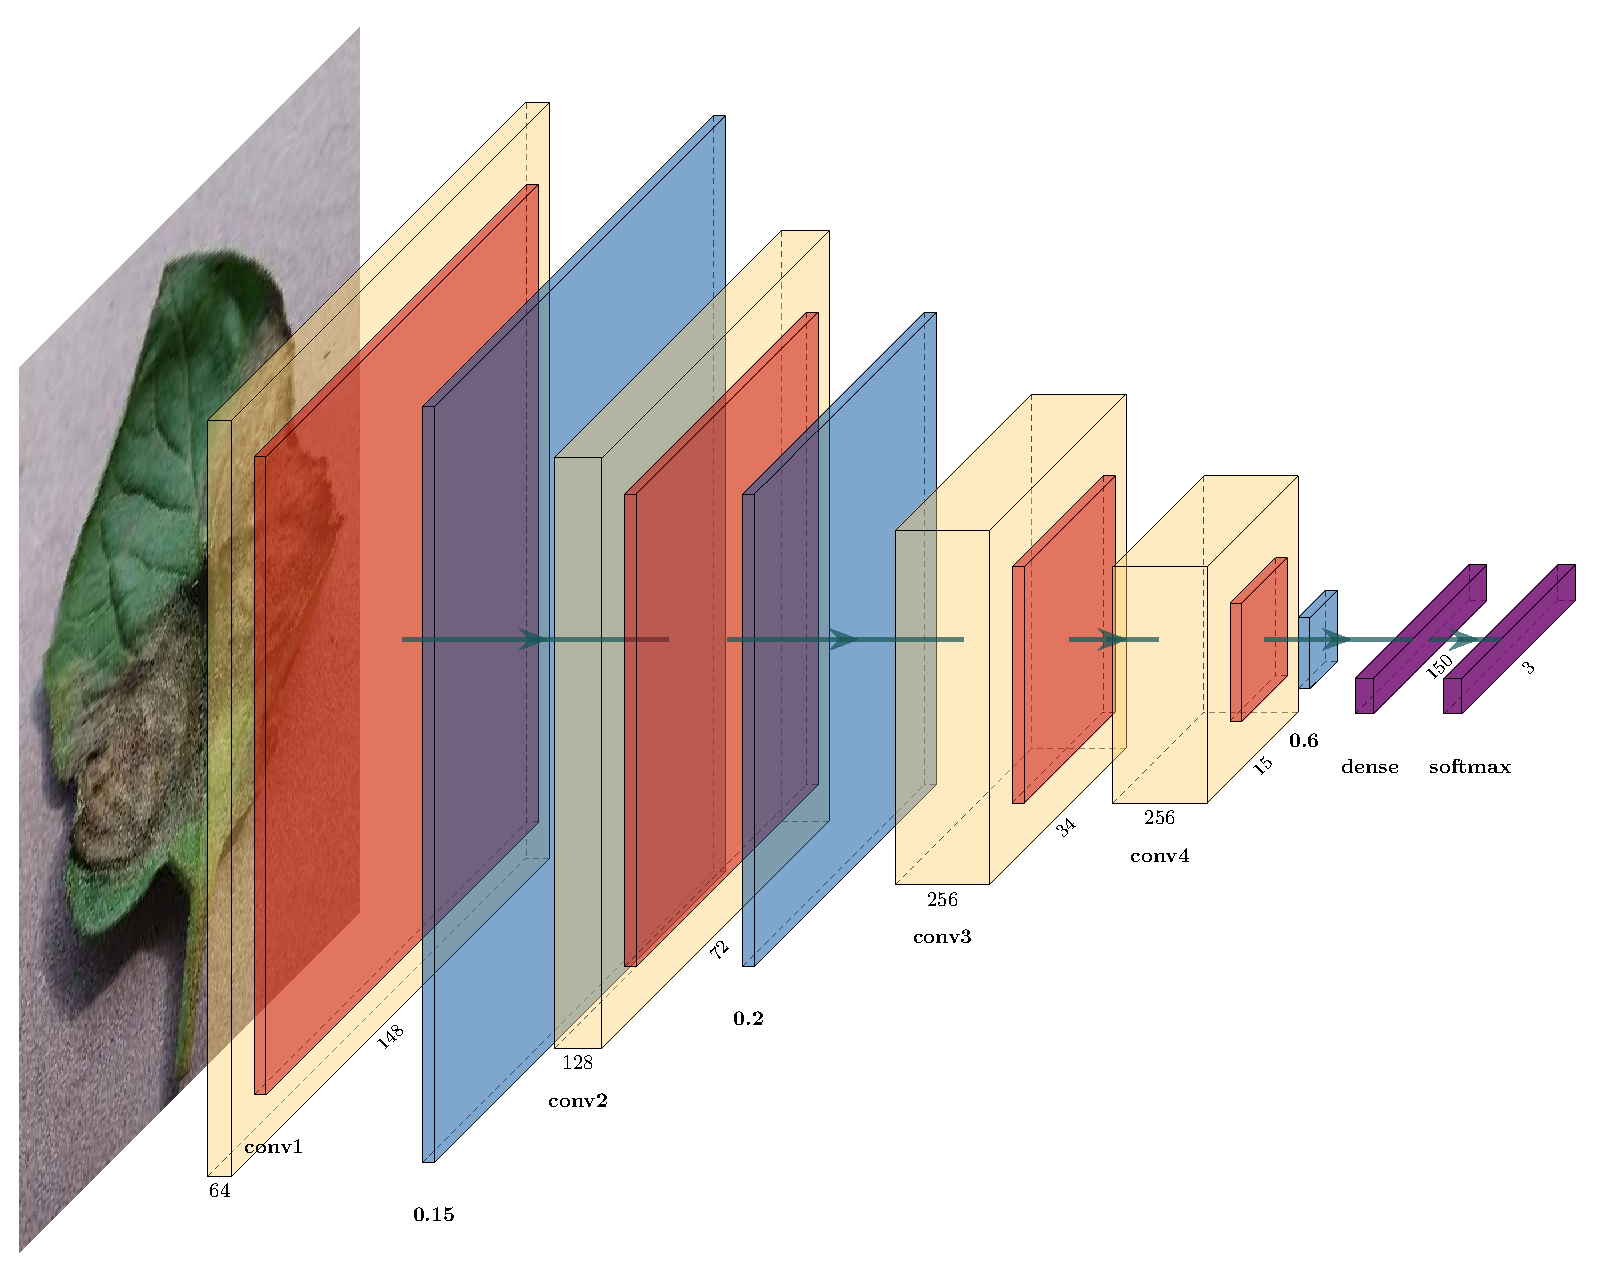
\includegraphics[width=\textwidth]{bilder/voter1.pdf}
	\caption{Veranschaulichung des ersten Modells mit vier Faltungs- und Poolingschichten und drei Dropout-Schichten (eigene Darstellung).}
	\label{voter1}
\end{figure}

\newpage
\paragraph{Training}
~\newline

Dieses Modell erreicht schnell gute Ergebnisse. Schon bei der 35. Epoche von 100 wurden die minimalsten Kosten erreicht und das Modell weist bei weiteren Epochen keine Verbesserungen auf. Deswegen wird das Training nach 15 weiteren Epochen abgebrochen. Die Genauigkeit des Modells liegt bei 97.94\%. 


\subsection{Modell 2}
\label{model2_voter}
%\subsubsection{Struktur}

Dieses Modell setzt auf viele Faltungsschichten mit einer kleinen Anzahl von Filtern. Die erste Faltungsschicht hat lediglich acht Filter. Die darauffolgende Dropout-Schicht ist auf den Wert 15\% eingestellt. Zwei weitere Dropout-Schichten, die in den nächsten zwei Iterationen von Faltungsschichten und Poolingschichten auftreten, sind auch auf den Wert 15\% konfiguriert. Nach der ersten Faltungs- und Poolingschicht folgt wieder eine Kombination, in der die Anzahl der Filter von acht auf 16 erhöht wurde. Die dritte Kombination mit 32 Filtern setzt sich nach der zweiten Dropout-Schicht fort. Erst auf die anschließende Kombination mit 64 Filtern nach der dritten Dropout-Schicht folgt eine weitere Dropout-Schicht, die ihre Rate von 15\% auf 20\% angepasst hat.

\begin{figure}[h!]
	\centering
	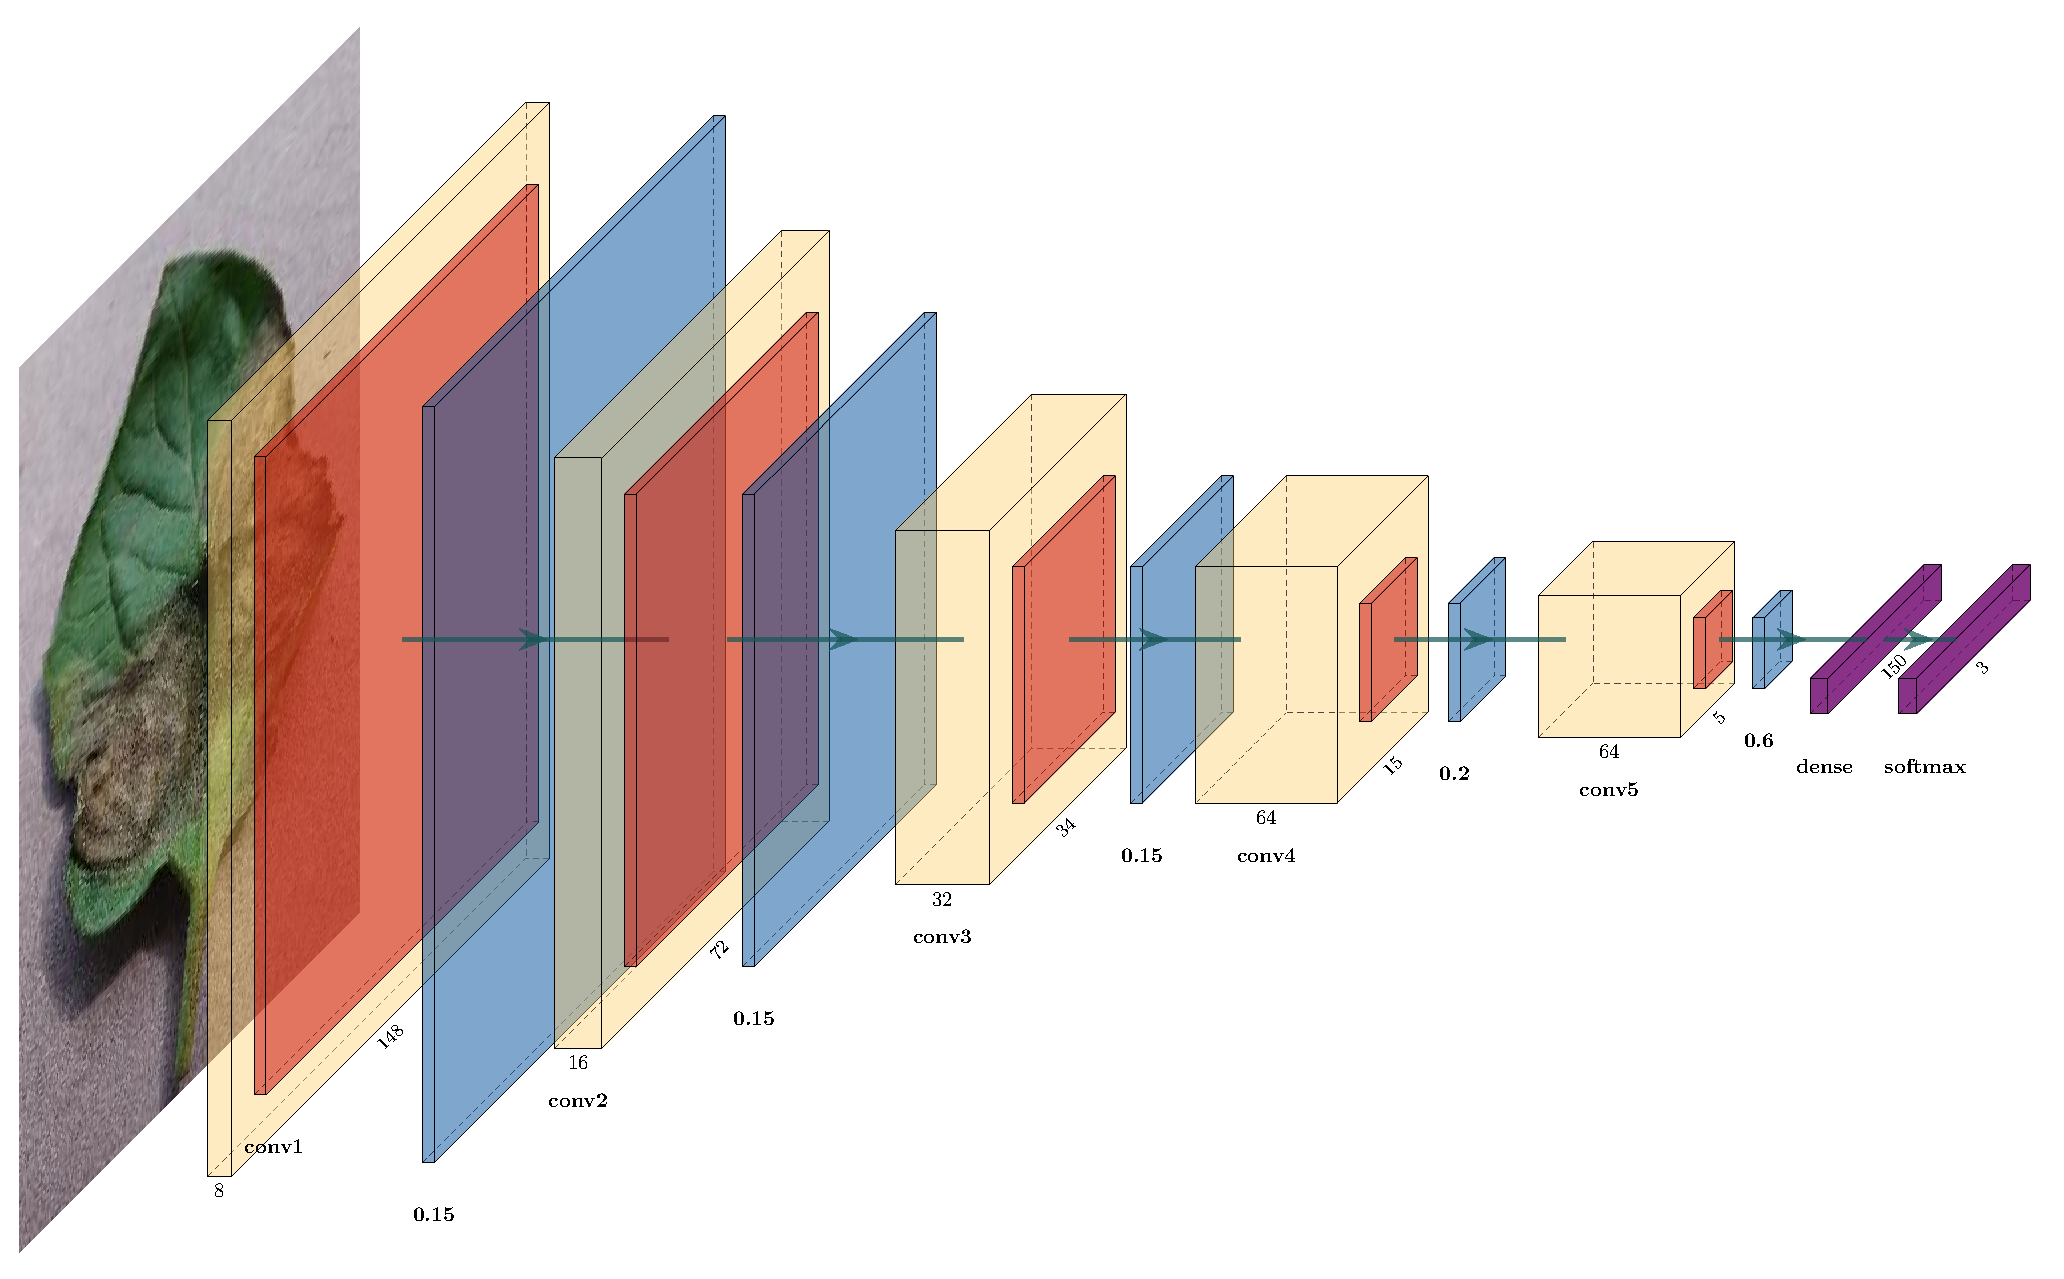
\includegraphics[width=\textwidth]{bilder/voter2.pdf}
	\caption{Veranschaulichung des zweiten Modells mit fünf Faltungs-, Pooling- und Dropout-Schichten (eigene Darstellung).}
	\label{voter2}
\end{figure}

Nun erhält die Architektur ihre letzte Kombination aus einer Faltungsschicht mit derselben Anzahl von Filtern und einer Max-Poolingschicht. Auch hier wird mit einer Dropout-Schicht, die die Rate von 60\% wie aus den Modellen \ref{sec:customNN} und \ref{model1_voter} bekannt ist, ergänzt. Letztendlich benötigt die Architektur des neuronalen Netzes noch zwei voll verbundene Schichten mit jeweils 150 und drei Knoten. Die erste voll verbundene Schicht verwendet die ReLU-Aktivierungsfunktion mit der L2-Regularisierung, die die Gewichte um den Faktor 0.002 berichtigt. Die letzte Schicht ist für die Klassifikation zuständig. Daher hat diese die Softmax-Aktivierungsfunktion.


~\newline
\paragraph{Training}
~\newline



Mit 100 Epochen wurde das Training dieses Modells gestartet. Des Weiteren wurde das Training so konfiguriert, dass nach 15 Epochen das Lernverfahren abgebrochen wird, wenn sich die minimale Kosten nicht verringern. Der Abbruch erfolgt bei der 92. Epoche, da die Kosten nicht kleiner werden. Das beste Modell bezüglich der minimalen Kosten wurde in der 77. Epoche gefunden und legt eine Genauigkeit auf dem Trainingsdatensatz von 96.54\% dar. 


~\newline
\subsection{Modell 3}
\label{model3_voter}
%\subsubsection{Struktur}

Ein weiteres Modell verwendet dieselbe Strategie des Modells \ref{model2_voter}. Hier wird auch auf viele Faltungsschichten gesetzt. Nach jeder Faltungsschicht mit der Max-Poolingschichtkomponente folgt eine Dropout-Schicht. Die erste Faltungsschicht nimmt wie bei allen anderen Modellen das Eingangsbild an und hat genau acht Filter. Anschließend folgt schon die erste Dropout-Schicht, die auf 15\% eingestellt ist. Nach diesem Muster wird die Architektur des neuronalen Netzes erstellt. Dies wird noch zwei mal wiederholt. Dabei verdoppelt sich iterativ die Anzahl der Filter in der Faltungsschicht. Des Weiteren sind bis dahin alle Dropout-Schichten auf den Wert 0.15 eingestellt. Die vierte Faltungsschicht hat genau so viele Filter wie die vorherige Faltungsschicht, nämlich 32. Daraufhin schließt sich die letzte Dropout-Schicht an, welche auf 60\% konfiguriert ist. Abschließend vervollständigt sich das Modell mit zwei voll verbundenen Schichten. Die erste folgende Schicht hat 150 Knoten mit der ReLU-Aktivierungsfunktion sowie L2-Regularisierung, die aus den anderen Modellen bekannt sind. Die letzte voll verbundene Schicht hat drei Knoten für die Klassifikation, die mittels der Softmax-Aktivierungsfunktion erfolgt.

\begin{figure}[h!]
	\centering
	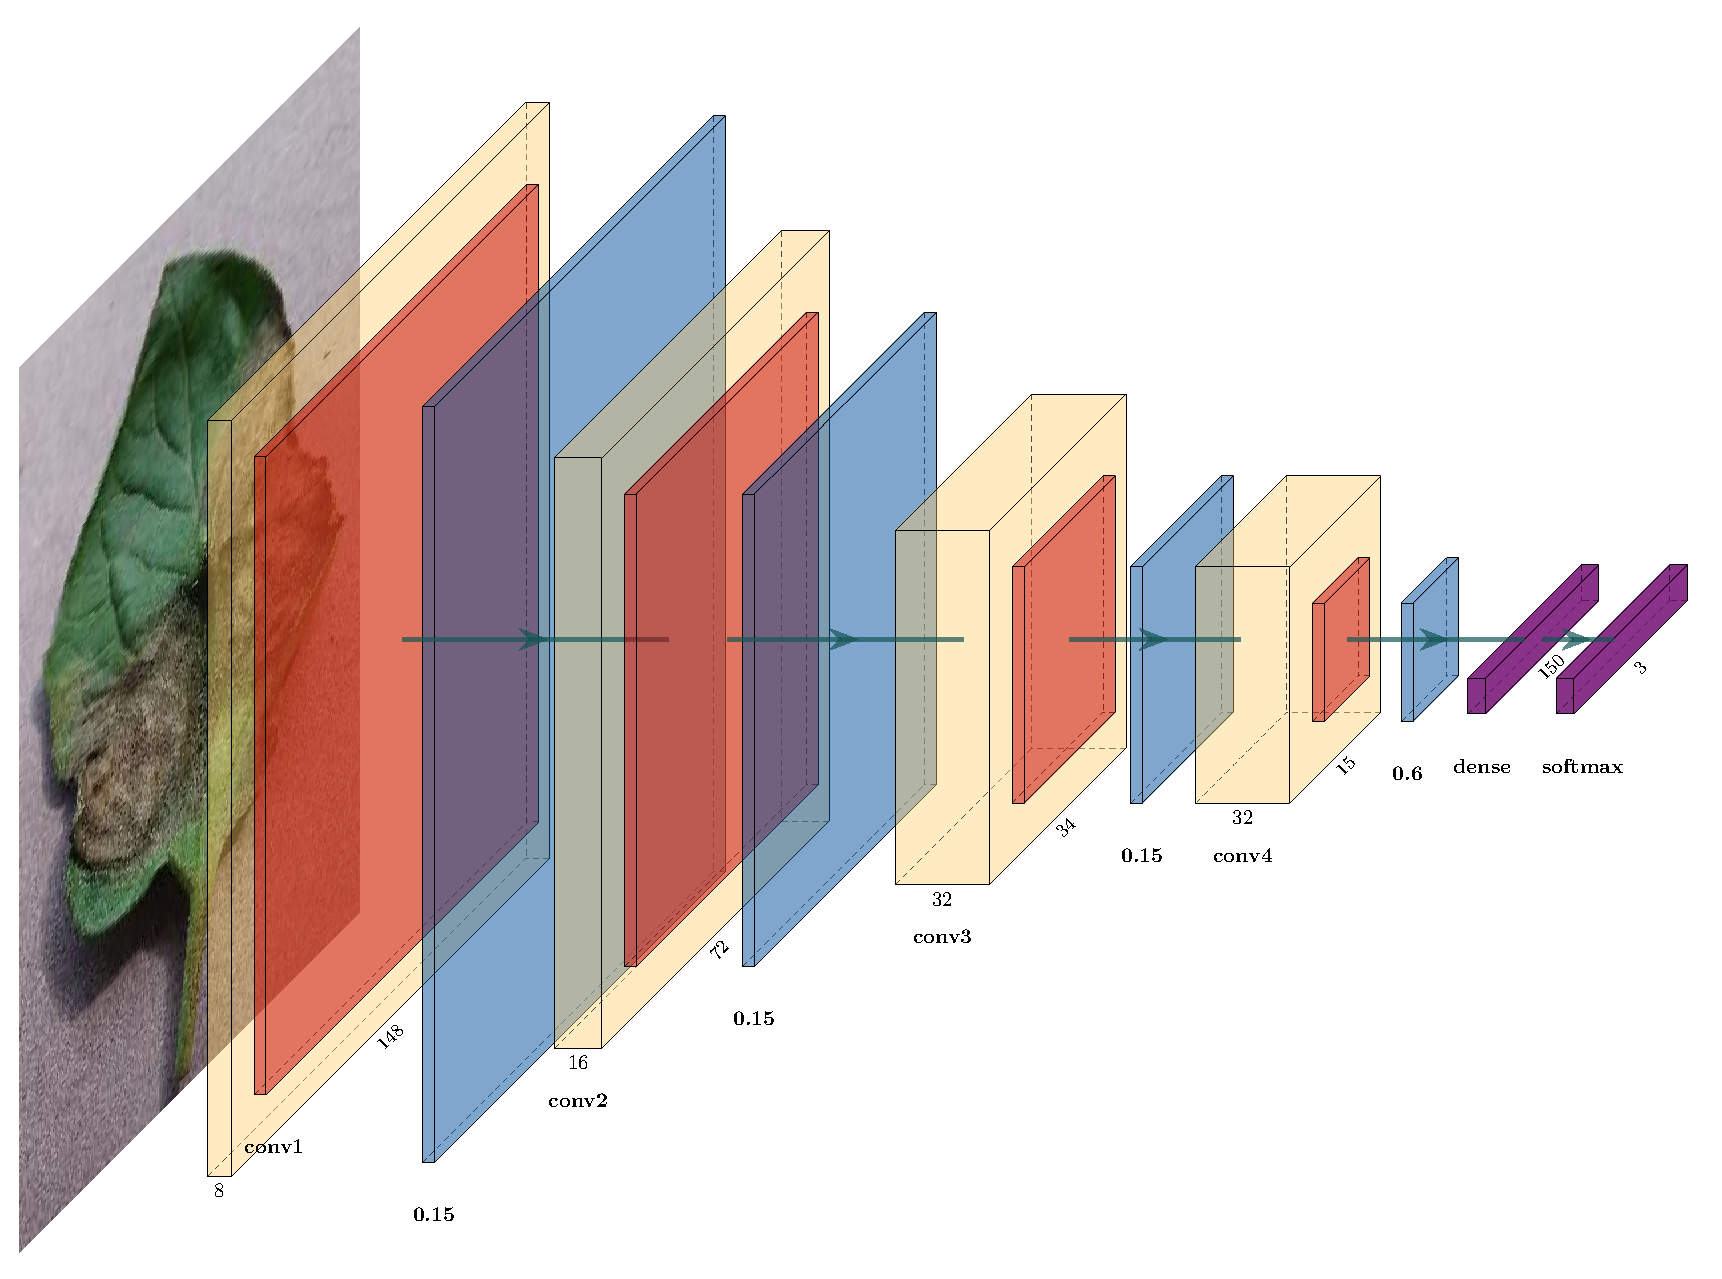
\includegraphics[width=\textwidth]{bilder/voter3.pdf}
	\caption{Veranschaulichung des dritten Modells mit vier Faltungs-, Pooling- und Dropout-Schichten (eigene Darstellung).}
	\label{voter3}
\end{figure}




\newpage
\paragraph{Training}
~\newline


Das Training des Modells wird auch hier mit 100 Epochen gestartet. Das Training wird abgebrochen, wenn nach 15 Epochen keine Verbesserung der Minimierung auftritt. Dies tritt bei der 79. Epoche ein. Das beste Modell bezüglich der minimalen Kosten wurde in der 64. Epoche entdeckt und die Genauigkeit liegt bei 96.92\%. 


\section{Transfer gelerntes Modell}
\label{sec:transferlearning}


Die Basisstruktur des folgenden neuronalen Netzes basiert auf der Grundlage des Lernens durch den Transfer von vortrainierten Modellen (engl. transfer learning). Die Idee dahinter ist, dass trainierte Modelle auf ein neues, aber verwandtes Problem angewendet werden. Solche Modelle werden in der Regel auf einem sehr großen Datensatz trainiert. Die gelernten einfachen Merkmale, zum Beispiel Formen und Figuren, werden wiederverwendet, um solche Repräsentationen nicht noch einmal trainieren zu müssen \cite{Subramanian2018,natural,Vasilev2019}. 



Da alle größeren vortrainierten Modelle keine Blattkrankheiten als Klassen haben, wird ein beliebiges, vortrainiertes Modell, hier VGG19\cite{VGG16}, verwendet. 

\begin{wrapfigure}{r}{5cm}
	\centering
	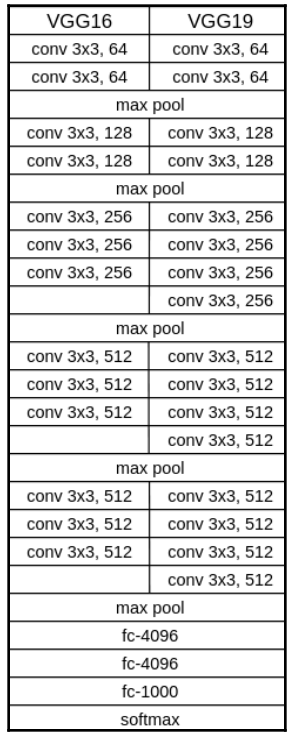
\includegraphics[width=0.18\textheight]{bilder/vgg19.PNG}
	\caption{Darstellung der VGG16 und VGG19 Struktur\cite{Vasilev2019}.}
	\label{VGG19_arch}
\end{wrapfigure}

Das neuronale Netzwerk besteht aus mehreren Blöcken, die mit zwei oder vier gestapelten Faltungsschichten in Kombination mit einer Max-Poolingschicht versehen sind. In Abbildung \ref{VGG19_arch} ist die Struktur der Architektur mit 16 und 19 Schichten visualisiert. Das Netzwerk hat bei zunehmender Tiefe deutlich mehr Filter in den Faltungsschichten. Die Anzahl der Filter reicht von 64 bis 512. Jede Faltungsschicht hat innerhalb eines Blocks dieselbe Anzahl von Filtern. Anschließend folgen drei voll verbundene Schichten. Davon sind zwei Schichten mit 4096 Knoten versehen. Die dritte Schicht hat 1000 Knoten\cite{Vasilev2019}. 


Um das vortrainierte Modell verwenden zu können, muss die letzte voll verbundene Schicht mit der Softmax-Aktivierungsfunktion entfernt werden. Nach der Entfernung werden zwei voll verbundene Schichten mit 150 und fünf Knoten hinzugefügt für die Klassifikation von fünf Klassen. Wichtig ist es zu beachten, dass die Gewichte des ursprünglichen VGG19-Modells eingefroren werden, um die extrahierten Merkmale aus dem großen Datensatz beibezuhalten. 


\paragraph{Training}
~\newline


Dieses Modell hat im Vergleich zu anderen Modellen die höchste Epochenanzahl, hier 150. Der Abbruch des Trainings erfolgt erst nach 35 Epochen bei einer Nicht-Verbesserung der minimalen Kosten. Dies geschieht bei diesem Modell ab der 103. Epoche. Die Genauigkeit des Modells beträgt 71.1\%. 



